\documentclass[12pt]{report}
\usepackage[pdftex]{graphicx}     
\usepackage{fancyhdr}
\usepackage{setspace}
\usepackage{sectsty}  

\usepackage{times}
\usepackage{mathptmx}
\usepackage{lscape}
\usepackage{float}
\usepackage[english]{babel}
\usepackage[T1]{fontenc}
\usepackage{etoolbox}
\usepackage[utf8]{inputenc}
\usepackage{geometry}
\usepackage{listings}
\usepackage{color}
\definecolor{lightgray}{rgb}{.9,.9,.9}
\definecolor{darkgray}{rgb}{.4,.4,.4}
\definecolor{purple}{rgb}{0.65, 0.12, 0.82}
\lstdefinelanguage{JavaScript}{
	keywords={break, case, catch, continue, debugger, default, delete, do, else, false, finally, for, function, if, in, instanceof, new, null, return, switch, this, throw, true, try, typeof, var, void, while, with},
	morecomment=[l]{//},
	morecomment=[s]{/*}{*/},
	morestring=[b]',
	morestring=[b]",
	ndkeywords={class, export, boolean, throw, implements, import, this},
	keywordstyle=\color{blue}\bfseries,
	ndkeywordstyle=\color{darkgray}\bfseries,
	identifierstyle=\color{black},
	commentstyle=\color{purple}\ttfamily,
	stringstyle=\color{red}\ttfamily,
	sensitive=true
}

\lstset{
	language=JavaScript,
	backgroundcolor=\color{lightgray},
	extendedchars=true,
	basicstyle=\footnotesize\ttfamily,
	showstringspaces=false,
	showspaces=false,
	numbers=left,
	numberstyle=\footnotesize,
	numbersep=9pt,
	tabsize=2,
	breaklines=true,
	showtabs=false,
	captionpos=b
}
\chapterfont{\centering}
\sectionfont{\fontsize{12}{15}}
\graphicspath{ {images/} }
\setcounter{secnumdepth}{5}

\pagestyle{fancy}
\fancyhf{} 
\lhead{\footnotesize Project Report 2016}
\chead{}
\rhead{\tiny Market Intelligence System}	%type your topic here
\lfoot{Department of CSE}
\cfoot{\thepage}
\rfoot{College of Engineering Trivandrum}
\renewcommand{\headrulewidth}{0.4pt}
\renewcommand{\footrulewidth}{0.4pt}
\linespread{1.3}

\begin{document}

\begin{abstract}
This project is aiming at providing information about the trending technologies and market watch to the common man. Data sources which are possible to contain information regarding the Technology updates are RSS Feeds and social media. Data is extracted from these sources. Collected articles from the websites are tagged according the contexts and taxonomies. Triplet relations are extracted from these articles using NLP. Stanford Core NLP, Alchemy are the tools used for processing the articles. Triplets obtained will be put in a graph database. A triplet represents the entity – entity – relationship model. Entities can be a Company, a Product, a Technology or an industry. Neo4j is the graph database used for this purpose. Finally by using the predefined graph traversals and querying intelligence such as Competitors of a product, company, technology and useful information such as location based searching for different companies can be easily obtained. A web console will be provided for manual searching using the D3.js library. We have also provided a webpage displaying technology and market trends, i.e., the data we are having in our database .Languages used will be Java and Python for data extraction, relation extraction, tagging etc. Node JS will be server side backend. Java Script for the web front end. Neo4j  PostgreSQL will be databases.
\end{abstract}

\pagenumbering{roman}
\clearpage
\addcontentsline{toc}{chapter}{\listfigurename}
\tableofcontents		
\listoffigures

\chapter{Introduction}
\pagenumbering{arabic}
\par
Significance of Artificial intelligence is increasing in the day to day life. Natural language processing is an important component of artificial intelligence. Natural Language Processing is an area of research and application that explores how computers can be used to understand and manipulate natural language text or speech to do useful things. Applications of NLP include a number of fields of studies, such as machine translation, natural language text processing and summarization, user interfaces, multilingual and cross language information retrieval (CLIR), speech recognition, artificial intelligence and expert systems, and so on. The technology that is going to rule the next generation is the text processing.
\par
The aim of this project is to collect the data that is spread across the web, and process in a better way, which can be used for updating knowledge of the mankind. In this project we are implementing a system, which keep track of the technology and market trends around the globe.
This comes under a broader view of Internet of Things. 
\par
We have built the system to accommodate two kinds of users, the corporate user and the naïve user. At the completion of this project we have managed to provide a website, through which the user can locate technology companies based on locations, their field of expertise. In this web portal, users can also find different companies sharing same geographic location and technology areas they are engaged in. We are also providing a website in which user can walk through the technology related articles.
\par
Market Intelligence using graph database project involves four modules. These modules are Data extractor module, NLP module, Middleware module, Frontend module. The data is spread across the web. In order to collect this data, we created the Data extractor module. The data of our interest are collected from RSS field. We have used Crunchbase API, Discovery API, Boilerpipe API, AngelList API for initial database creation and data extraction.
\par
In the Natural language processing module, we extract the relations and keywords from the data that we have collected from the web using our extraction module. We have used Alchemy API for relation and keyword extraction. The keywords used for processing are launch, announcement, merging, invest, introduce, patent, appoint, hire etc. The output of the NLP module is used for tagging articles.
\par
The next module that is the middleware module operate on the output from the previous module.
In this module, we check whether the data that we have extracted satisfies out grammar constraints. Any data that does not match any constraints are excluded. If it matches any of the constraint, it will be sent to the admin for validation. Another task of this module, is to avoid certain entities so that we are able to represent only the required ones in the graph. 
\par
The frontend module is another important module in this project. Our frontend module conforms to the golden rules of user interface design. We have created two websites, one for the user to query and the other one for displaying technology articles. In the user website, we provide the privilege for the user to create queries of his needs and query in our database. By enabling this feature, we have manages to put the user in control. The output of the query is displayed using graph. To realize this, we make use of the D3 visualization library. During the development of all these modules, we have managed to conform to industry standards.
\par
The project aims at redefining the way the knowledge is made available for the common and corporate people, in a much convenient and easier to access way. We have tried at our level best in making sure that only legit information is made available to the users.


\chapter{Requirement Analysis}
\section{Software requirement specification}
\subsection{Introduction}
\subsubsection{Purpose}
\par The purpose of this document is to provide a description of the ‘Market Intelligence using Graph database’. This system aims to build a graph database of different companies,  their products and the technologies on which they are working on. This document provides a detailed description of the features, working, requirement and scope of the product. It is intended for reference by users of the software and for those interested in studying the working of the system.
\subsubsection{Document convention}
Main Section Titles
\begin{itemize}
	\item Font: Times New Roman
	\item Face: Bold
	\item Size: 14
\end{itemize}
Sub Section Titles
\begin{itemize}
	\item Font: Times New Roman
	\item Face: Bold
	\item Size: 12
\end{itemize}
Other Text Explanations
\begin{itemize}
	\item Font: Times New Roman
	\item Face: Plain
	\item Size: 12
\end{itemize}
\subsubsection{Intended Audience and Reading Suggestions}
This Software Requirements Specification document is intended for:
\begin{itemize}
\item Developers who can review project’s capabilities and more easily understand where their efforts should be targeted to improve or add more features to it (design and code the application – it sets the guidelines for future development).
\item Project testers can use this document as a base for their testing strategy as some bugs are easier to find using a requirements document. This way testing becomes more methodically organized.
\item End users of this application who wish to read about what this project can do.
\end{itemize}
It is suggested to go through the document in the same sequence as it is written.
\subsubsection{Product scope}
\par This software system will finally create a graph database of companies, their products and the technologies in which these companies are working in. This software will be used by different company officials who are interested in knowing the different market movements and updates. Software will be provided as a SAAS platform in which the users can view the required portions of the graph and see their connections and updates. Querying the graph is allowed by the software which can help in navigating the nodes and associated relations. Users can identify the competitors of a product, company and companies working in a specific platform. It also shows the recent announcement of the company and news articles related to the company product info in the graph. It can also be used by different investors to help investing in successful firms according to the locations of the firm, recent advancements of the firm etc.
\subsection{Overall description}
\subsubsection{Product perspective}
\par This project Market intelligence using graph data is an entirely new product in this arena.   No other organization have come up with this sort of idea so far. This project have an over evolving database. In the coming years, text processing have unlimited possibilities database can be used to process corporate data according to the clients need. This project can perform in Business to Business basis
\subsubsection{Product functions}
\par The major part of this project is to process the corporate data. The data is fetched from
news articles and RSS feeds. Software’s will be provide provided as a SAAS platform in which the users the graph is allowed by the software see their connections and updates. Querying the graph is allowed by the software which can help in navigating the nodes and associated relations. Users can identify the competitors of a product, company and companies working in a
specific platform.
\subsubsection{User characteristics}
\par The users of this project are corporates and naïve users. Users can query the graph is allowed by the software which can help in navigating the nodes and associated relations. Users can identify the competitors of a product, company and companies working in a specific platform.

\subsubsection{Operating Environment}
Client:
\begin{itemize}
\item Software:
\begin{itemize}
\item Ubuntu 12.04
\item Windows XP and above
\end{itemize}
\item Hardware:
\begin{itemize}
\item RAM 2GB
\item Intel Core i3 processor and above
\end{itemize}
\end{itemize}
Server:
\begin{itemize}
\item Software:
\begin{itemize}
\item Ubuntu 14.04
\item Neo4j 2.2
\item Postgres 9.4
\item Java JDK 7
\end{itemize}
\item Hardware:
\begin{itemize}
\item RAM 8GB
\item HDD 8GB
\end{itemize}
\end{itemize}

\subsubsection{Design and implementation constraints}
\par The main design implementation difficulty is limitation of Natural language processing tools to extract the exact relations. Another difficulty is in processing eliminating the junk in the data obtained from websites.
\subsubsection{Assumption and dependency}
\par Our assumptions are the data obtained from news websites are legit and in format as we expect.

\subsection{External Interface Requirements}
\subsubsection{User Interface}
\par We provide a webpage in which the user can query different possibilities. A graph will be embedded in the webpage where users can query graphically. We also provide a website to display the recent activities taking place in the technology world.

\subsection{System Features}
\begin{itemize}
\item Dynamic and static data collection methods are built. Static data collector updates once in 2 or 3 months,while the dynamic collector will run every day.
\item Feed fetcher will parse the RSS feeds and extract the link. Rome API is used for this.
\item Webpage content extractor will fetch the news content from the webpage eliminating all garbages present in website. Google's Boilerpipe API is used for this.
\item NLP is the core module of this project. This will extract the entities as well as relations from the news website. This will be given to the graph updater. Graph updater will remove redundant relations and update it in the graph.
\item Neo4j is used as the graph database.PostgreSQL is used as live db which holds other informations
\end{itemize}

\subsection{Other Non-functional requirements}
\subsubsection{Performance requirements}
For operation involving graph querying especially when the number of nodes grows linearly with time, the system needs good processing power to perform in real-time. This requires  the installation of large main memories.

\subsubsection{Safety requirements}
\par There is no safety issues if this project is implemented correctly.
\subsubsection{Security Requirements}
\par Care should be taken to avoid any vulnerabilities in the website. The data obtained from feed fetch module must be correctly entered into the database. Since the accuracy of the NLP module is not certain, there will be privilege for the administrator to crosscheck the entries to the database.
\subsubsection{Business Rules}
\par During the initial training phase, operations are not done on the data fetched. We manually enter data, process it using NLP module and enter the data onto the graph database.

\subsection{Other Requirements}
\par Almost all requirements have been included earlier. If any, to be added further will be informed later.

\chapter{Project Design}
\section{Use Case Diagram}
\begin{figure}[h]
	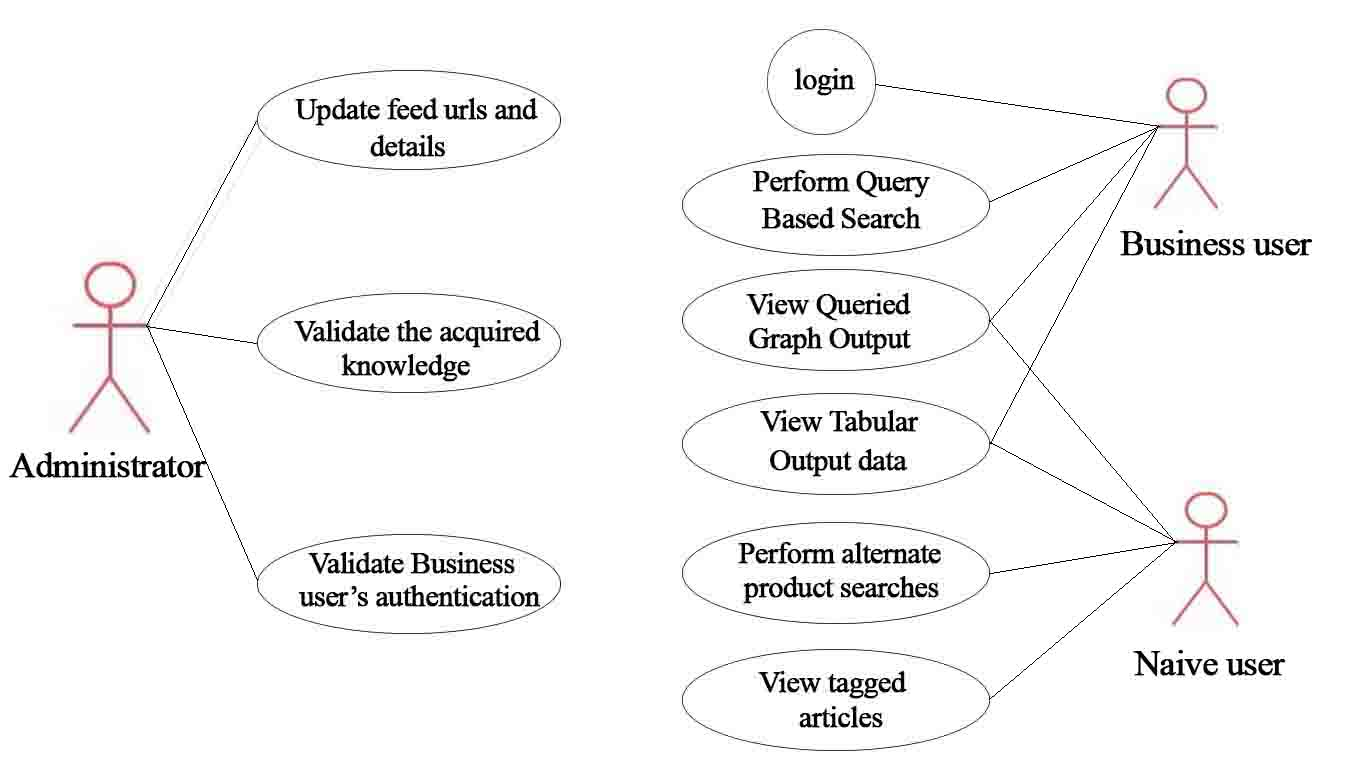
\includegraphics[width=13cm, height=7cm]{usecase}
	\centering
	\caption{Use case Diagram}
\end{figure}
\newpage
\section{Data Flow Diagram}
\begin{figure}[h]
	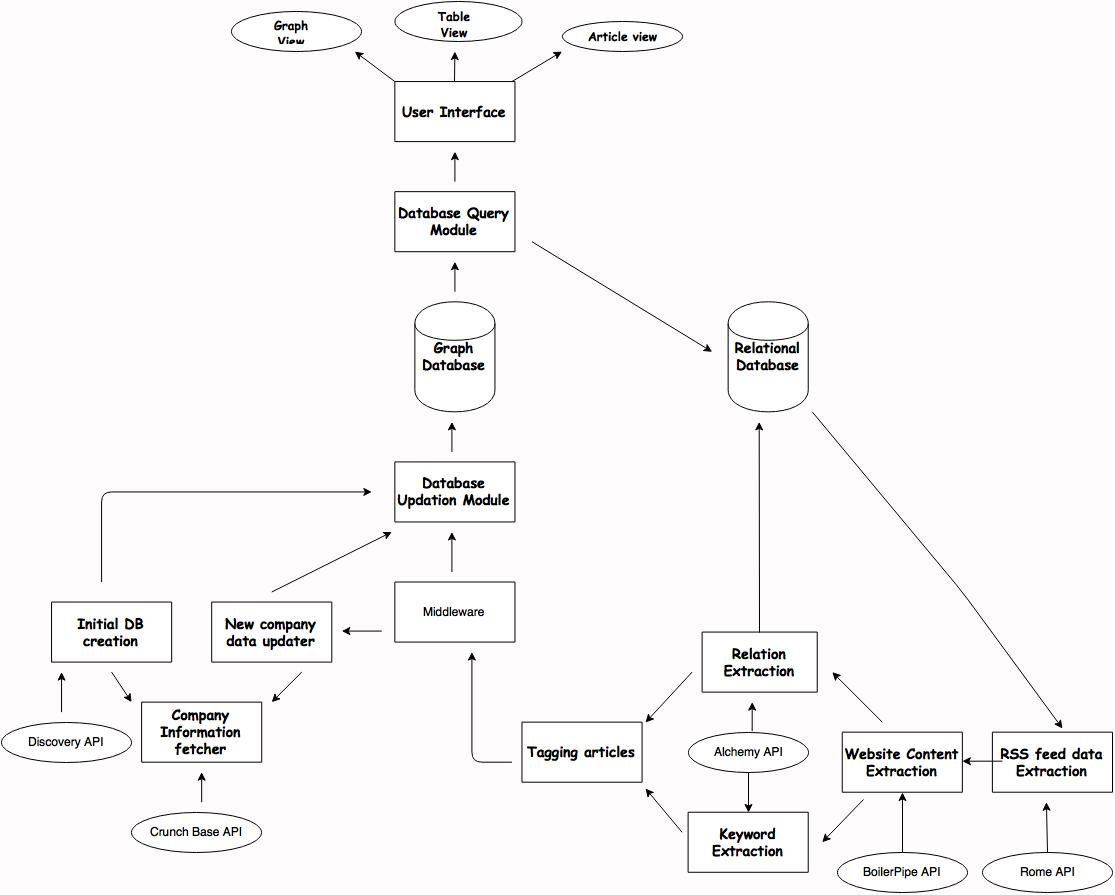
\includegraphics[width=10cm, height=11cm]{dataflow}
	\centering
	\caption{Data Flow Diagram Diagram}
\end{figure}
\newpage
\section{Database design}
\par There are two types of database systems used they are 
\begin{itemize}
\item Graph database 
\item Object-Relational database
\end{itemize}

\subsection{Graph database}
\par 
In computing, a graph database is a database that uses graph structures for semantic queries with nodes, edges and properties to represent and store data. A key concept of the system is the graph (or edge or relationship), which directly relates data items in the store. This contrasts with conventional relational databases, where links between data are ad hoc and based on the data itself, and related items are gathered by searching for this data within the store. Graph databases are designed to allow simple and rapid retrieval of complex hierarchical structures, whereas a relational database would use a complex query to achieve the same end, generally with far less performance.\cite{graphvisualiztion}
\par The underlying storage mechanism of graph database products varies. Some, like Maria DB, are based on a relational engine and store the graph data in a table. More common examples generally use a key-value store or document-oriented database for storage, making them inherently NoSQL solutions. These solutions generally offer a performance advantage because the graph is stored in a format similar to a database index, minimizing its size and retrieval time. Most graph databases based on non-relational storage engines also add the concept of tags or properties, which are essentially relationships lacking a pointer to another document. This allows data elements to be categorized for easy retrieval in mass. Examples of NoSQL graph databases include Orient DB, Neo4j and Arango DB.
\par The Graph database in use is Neo4j. It is a graph database management system developed by Neo Technology, Inc. Described by its developers as an ACID-compliant transactional database with native graph storage and processing, Neo4j is the most popular graph database according to db-engines.com.
\par Neo4j is available in a GPL3-licensed open-source "community edition", with online backup and high availability extensions licensed under the terms of the Affero General Public License. Neo also licenses Neo4j with these extensions under closed-source commercial terms.
\par Neo4j is implemented in Java and accessible from software written in other languages using the Cypher Query Language through a transactional HTTP endpoint.
 \par The graph database schema in use is depicted in the Figure \ref{fig:graphdatabaseschema}

\begin{figure}[h]
	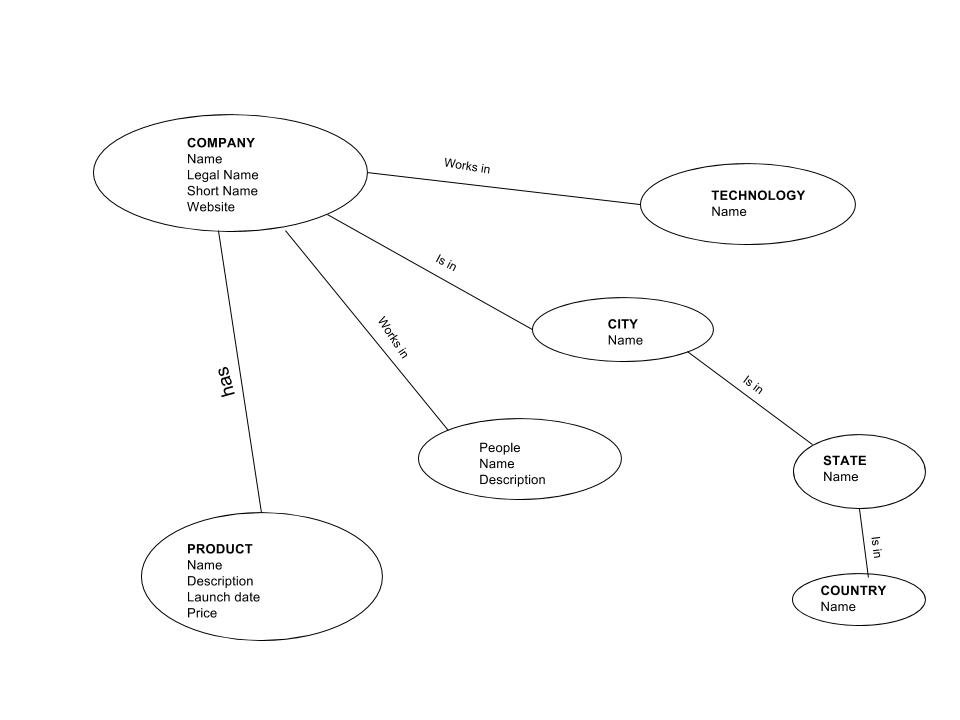
\includegraphics[width=10cm, height=11cm]{graphdatabaseschema}
	\centering
	\caption{The graph database schema}
	\label{fig:graphdatabaseschema}
\end{figure}

\subsection{Object-Relational database system}

\par An object-relational database (ORD), or object-relational database management system (ORDBMS), is a database management system (DBMS) similar to a relational database, but with an object-oriented database model: objects, classes and inheritance are directly supported in database schemas and in the query language. In addition, just as with pure relational systems, it supports extension of the data model with custom data-types and methods.
\par An object-relational database can be said to provide a middle ground between relational databases and object-oriented databases (object database). In object-relational databases, the approach is essentially that of relational databases: the data resides in the database and is manipulated collectively with queries in a query language; at the other extreme are OODBMS’s in which the database is essentially a persistent object store for software written in an object-oriented programming language, with a programming API for storing and retrieving objects, and little or no specific support for querying.
\par The ORDBMS in use is PostgreSQL, often simply PostgreSQL, is an object-relational database management system (ORDBMS) with an emphasis on extensibility and standards-compliance. As a database server, its primary function is to store data securely, supporting best practices, and to allow for retrieval at the request of other software applications. It can handle workloads ranging from small single-machine applications to large Internet-facing applications with many concurrent users.
\\
\par PostgreSQL implements the majority of the core SQL: 2011 standard, is ACID-compliant and transactional (including most DDL statements) avoiding locking issues using multi version concurrency control (MVCC), provides immunity to dirty reads and full serializability. handles complex SQL queries using many indexing methods that are not available in other databases; has updateable views and materialized views, triggers, foreign keys; supports functions and stored procedures, and other expandability, and has a large number of extensions written by third parties. In addition to the possibility of working with the major proprietary and open source databases, PostgreSQL supports migration from them, by its extensive standard SQL support and available migration tools. Proprietary extensions in databases such as Oracle can be emulated by built-in and third-party open source compatibility extensions. Recent versions also provide replication of the database itself for availability and scalability.
\par
PostgreSQL is cross-platform and runs on many operating systems including Linux, FreeBSD, OS X, Solaris, and Microsoft Windows. On OS X, PostgreSQL has been the default database starting with Mac OS X 10.7 Lion Server, and PostgreSQL client tools are bundled within the desktop edition. The vast majority of Linux distributions have it available in supplied packages.
\par PostgreSQL is developed by the PostgreSQL Global Development Group, a diverse group of many companies and individual contributors. It is free and open-source software, released under the terms of the PostgreSQL License, a permissive free-software license.
\par The schemas of the relations used in PostgreSQL are
\begin{itemize}
\item Feed (feed\_id, url, last\_accessed\_time)
\item Article (url, heading, taxonomy, context)
\item Temporary\_Relation (id, statement, subject\_text, subject\_text, object\_text, object\_type, verb\_text, context) 
\item Relations (relation\_id, statement, subject\_text, subject\_text, object\_text, object\_type, verb\_text, context) 
\item Taxonomy\_word (word, taxonomy)
\item Context\_work (word, context)
\item Taxonomy\_code (code, taxonomy)
\item Context\_code (code, context)
\item Company (website, name, legal\_name, short\_name)
\item Technology (name)
\item Works\_in (website, name)
\item City (name)
\item State (name)
\item Country (name)
\item Is\_at (website, name)
\item Is\_in (name, name)
\item Product (product\_id, name, launch\_date, description, price)
\item Has (website, product\_id)
\item Person (person\_id, first\_name, second\_name, designation)
\item Works\_in (person\_id, website)
\end{itemize}

\section{User interface design}
\par 
User interface is the front-end application view to which user interacts in order to use the software. User can manipulate and control the software as well as hardware by means of user interface. Today, user interface is found at almost every place where digital technology exists, right from computers, mobile phones, cars, music players, airplanes, ships etc.
\par User interface is part of software and is designed such a way that it is expected to provide the user insight of the software. UI provides fundamental platform for human-computer interaction.
\par UI can be graphical, text-based, audio-video based, depending upon the underlying hardware and software combination. UI can be hardware or software or a combination of both.

The software becomes more popular if its user interface is:
\begin{itemize}
\item Attractive
\item Simple to use
\item Responsive in short time
\item Clear to understand
\item Consistent on all interfacing screens
\end{itemize}
UI is broadly divided into two categories:
\begin{itemize}
\item Command Line Interface
\item Graphical User Interface
\end{itemize}
\subsection{Different user interfaces}
\par There are three separate user interfaces implemented for the use of different kinds of users they are 
\begin{itemize}
\item Naïve user
\item Business user
\item Administrator
\end{itemize}
\subsubsection{For the naive user}
\par The list of all articles that has been fetched by Dynamic data collector is listed here for the naïve user’s reference this is categorized according to their tags.  A synopsis of the article is provided in here itself, the interested user can follow the link to the original article.
\subsubsection{For the business user}
\par The business user can query the graph database to get a variety of predefined relations. The results may be shown either as the graph visualization or as a tabular representation according to the type of query.
\subsubsection{For the administrator}
\par The administrator interface lists the relations that are extracted by the Dynamic data extractor. Each relations will have subject, subject type, object, object type predicate, and predicate type. The sentence from which these relations are extracted are shown for verification. This will allow the filtering of duplicate as well as junk data.

\chapter{Implementation}
\section{Module 1 - Data Collection}
\par Like in any other system that deals with data processing, the prime component of the market intelligent system is the data. Data here refers to the information regarding the concerned companies and products that are gathered though various means.\\
Data collection for the system is done in two phases
\begin{itemize}
\item Initial Database Creation
\item Dynamic Data Collection
\end{itemize}
\subsection{Initial Database Creation}
\par To start with, we need to accumulate details regarding existing companies, their products and other relevant information. Working on an area like Technology, we are particularly interested in the following kinds of details regarding a company.
\begin{itemize}
\item Registered name
\item Launched products
\item Locations 
\item Associated and relevant people
\item Website information
\item Contact information
\item Acquisition details
\end{itemize}
\par Initial Database creation is a one-time process in the entire lifecycle of the system. It is meant to provide an initial database platform for the dynamic data updation procedure that follows. The data collection is done through various API modules available.

\subsubsection{Collecting Company Names}
\paragraph*{Clearbit’s Discovery API v1.0}
\hfill \break 
The first and foremost step is to make a list of companies working in the field that we are concerned with. The Discover API by Clearbit is used for this purpose. It helps to create a targeted list of companies using an advanced search parameter. The main 	features behind the selection of Discovery API for the purpose are.	

\begin{itemize}
\item Flexible API \\ Create lists of prospects for internal use or integrate the API directly into the system
\item Fast \\ It is considered to be relatively fast and light weighed when compared to counter options.
\item Reliable and Growing database. \\The database is constantly growing, up-to-date and is reliable.
\end{itemize}
\paragraph*{API invocation format}
\hfill
\par The calls to the API module are done as rest calls, passing the field of interest as the parameter.
\paragraph*{API response format}
\hfill \break
The response to the rest call is received in json format and need to be parsed to obtain individual company names.
\begin{figure}[h]
	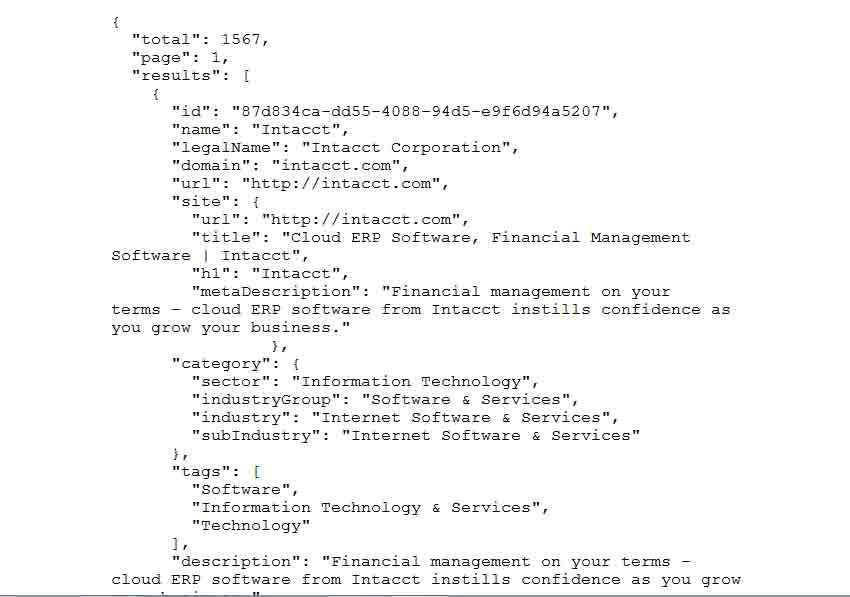
\includegraphics[width=15cm, height=12cm]{discovery1}
	\centering
	\caption{Response format of Discovery API Part1}
\end{figure}
\begin{figure}[h]
	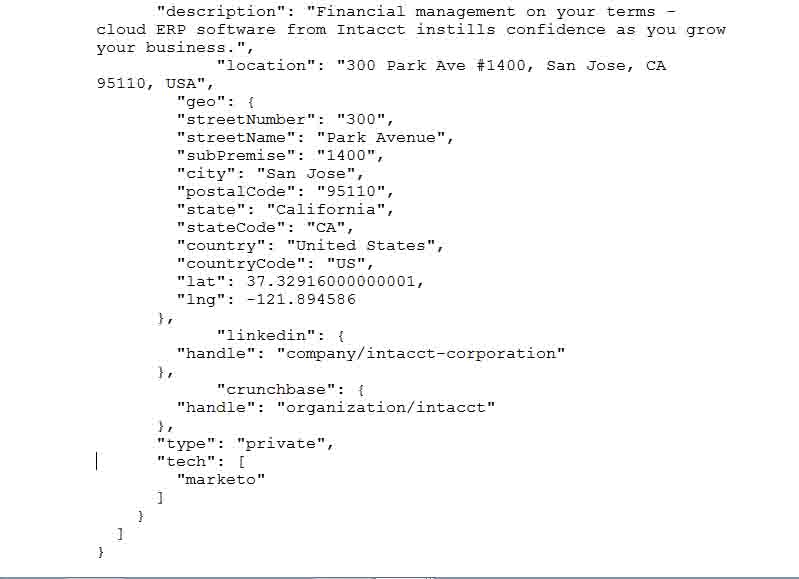
\includegraphics[width=15cm, height=12cm]{discovery2}
	\centering
	\caption{Response format of Discovery API Part2}
\end{figure}
\subsubsection{Collecting Company Details}
\paragraph*{CrunchBase API v2.0}
\hfill \break
The CrunchBase API gives developers, access to query the CrunchBase Dataset for both paginated lists of specific types of Items (e.g., Companies) and details about individual Items (e.g., the properties and relationships of a specific Company).
Developers can navigate through the Dataset by retrieving and inspecting individual Items and their relationships. Each detailed Item response includes not only the properties of the Item (e.g., a Company's name, founding date, and profile image) but also a list of all of its relationship types (e.g.,"competitors","current team").\cite{clearbit}
\paragraph*{API invocation format}
\hfill \break
The calls to the API module are done as rest calls, passing the company name as the parameter.
\paragraph*{API response format}
\hfill \break
The response to the rest call is received in json format and need to be parsed to obtain tabulated details of each company.
\begin{figure}[h]
	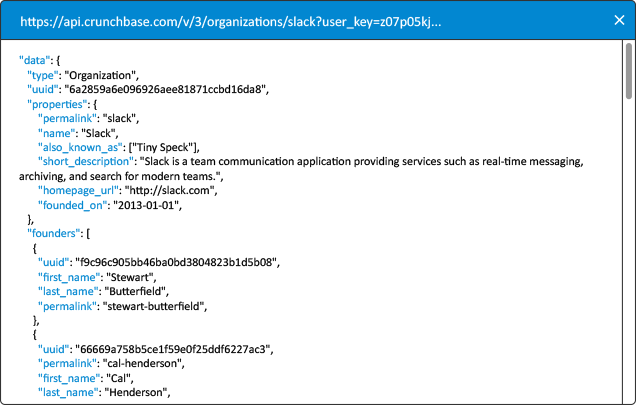
\includegraphics[width=12cm, height=8cm]{crunchbase}
	\centering
	\caption{response format of CrunchBase API}
\end{figure}
\par
The API allows only a limited number of calls to be made per account holder per hour. Hence the calls need to done as a scheduled task considering this limitation. Also, the process of retrieving the individual company details using the API might take a time delay of approximately two seconds per call. As a result, making calls in a sequential manner isn’t the best of options. This limitation is overcome by the application of multithreaded approach to API calls where concurrent calls and made at a time, collecting information regarding different companies.
\begin{figure}[h]
	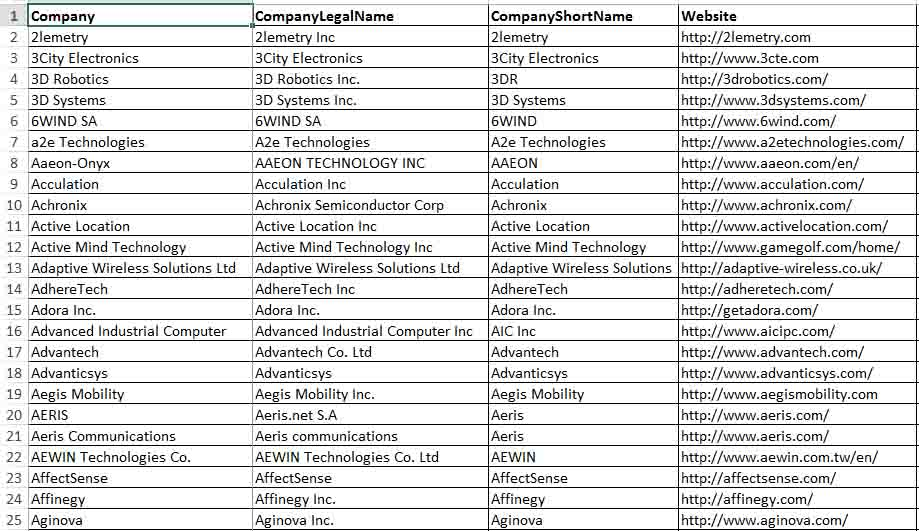
\includegraphics[width=15cm, height=10cm]{initial_db1}
	\centering
	\caption{Miniature tabulated format of details collected - part 1}
\end{figure}
\begin{figure}[h]	
	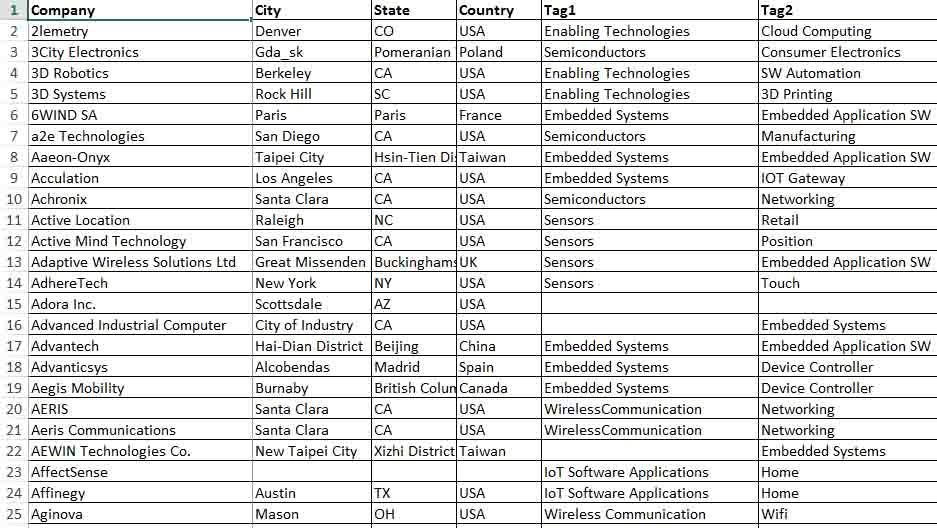
\includegraphics[width=15cm, height=10cm]{initial_db2}
	\centering
	\caption{Miniature tabulated format of details collected - part 2}
\end{figure}

\subsection{Dynamic Data Collection}
\par Once the initial database is created, it is required to make dynamic updation of data in order to incorporate the latest trends and happenings in the area (eg: Technology) concerned. This is done by extracting the relationships from articles and data made available from RSS feeds. The selection of reliable and consistent RSS feeds is done by the administrator. The extraction of details provided by the feeds is done by ROME API.
\subsubsection{Extraction from RSS feeds}
\paragraph*{ROME API}
\hfill \break
Rome is based around an idealized and abstract model of a Newsfeed or "Syndication Feed". Rome can parse any format of Newsfeed, including RSS variants and Atom, into this model. Rome can convert from model representation to any of the same Newsfeed output formats. Here we use the API module to parse the response provided by the feed in XML/Atom format.\cite{romeapidocs}

\paragraph*{API invocation format}
\hfill
\par The calls to the API module is done by passing the xml/atom file to the module.
\paragraph*{API response format}
\hfill \break
The API responds by providing an object that contains the parsed details of the concerned field. This contains the URLs to the articles as well as their short titles.
\begin{figure}[h]
	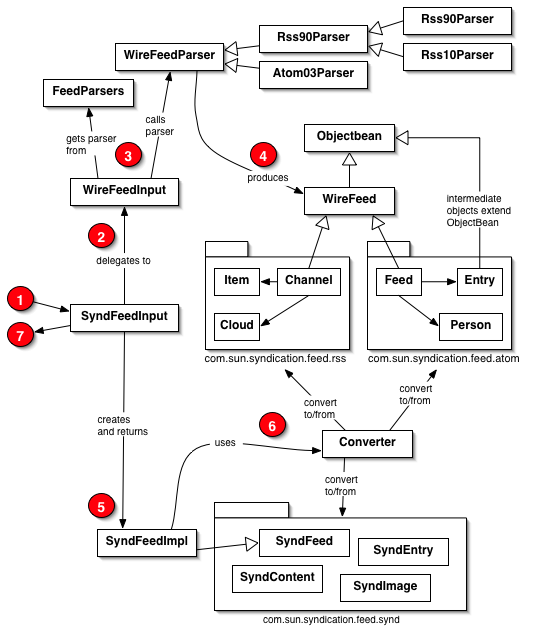
\includegraphics[width=10cm, height=11cm]{HowRomeWorks}
	\centering
	\caption{Internal working diagram of ROME API}
\end{figure}
\par When we are done collecting the URLs for the articles, the next step is to retrieve the text articles from the concerned URLs. 

\subsubsection{Extracting article text}
\paragraph*{Boilerpipe API}
\hfill \break
The URLs to articles return a page containing the concerned article as well as other elements such as advertisements, hyperlinks to other pages, promotional details etc. For the extracted data to be of some value, it is needed to retrieve only the potential article text from the URL and Boiler pipe API serves this need.
\paragraph*{API invocation format}
\hfill
\par The calls to the API module is done by passing the concerned URL to the module.
\paragraph*{API response format}
\hfill \break
The API responds by providing an object that encapsulates the article details and can be used to retrieve the text article for further processing.
\begin{figure}[h]
	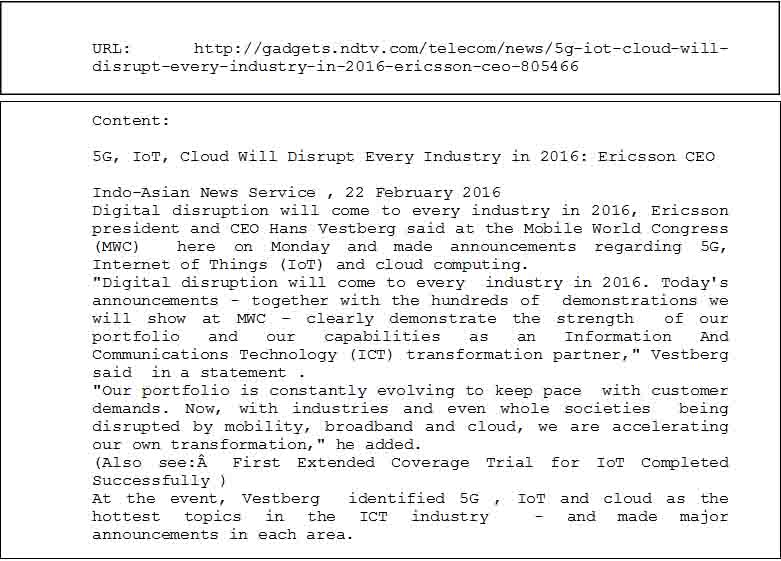
\includegraphics[width=10cm, height=8cm]{boilerpipe}
	\centering
	\caption{An example of passed URL and extracted text by Boilerpipe API}
\end{figure}

\section{Module 2 - Data Processing}
\par
For the retrieved articles to be incorporated to the existing database, it is needed to derive possible relations out of the articles and tag them accordingly. Data processing phase is aimed at providing this service. 
\paragraph*{Input to the phase:}
The article in text format is served as input to the data processing phase.
\paragraph*{Output from the phase:}
Consistent relationships involving concerned companies, products and their relationships are derived in the form of triplets (subject, object, verb).

\subsection{Initiating Context vocabulary}
\par The administrator need to establish a table with all the possible verb terms we are interested in the relation and those which are expected to be identified by the API module. This is to identify the context of each article and categorize them accordingly.
\\ A minimized list of contexts can be identified as 
\begin{itemize}
\item Tech Invest	
\item R\&D	
\item New Product Introduction	
\item Executive Moves	
\item Outsourcing And Offshoring	
\item Contracts Central	
\item Technology In Action	
\item Intellectual Property Rights	
\item Talent Tracker
\item M\&A Tracker
\end{itemize}

\subsection{Initiating Taxonomy vocabulary}
\par It is also required to maintain a table containing the taxonomy terms we are interested in. This is to relate the keywords extracted by the API with each taxonomy terms and tag articles accordingly.
\\
A minimized list of taxonomies can be identified as
\begin{itemize}
\item Social Networks
\item Social Media
\item Social Trends	
\item Social Challenges	
\item Mobile Devices	
\item Mobile Networks	
\item IoT	
\item Mobile Apps
\item Big Data	
\item Business Analytics	
\item Location Analytics	
\item Information Management	
\item Cloud Infrastructure	
\item Cloud Computing	
\item Saas/PaaS/IaaS	
\item Virtualization
\end{itemize}

\subsection{Defining Grammars}
\par To make the system work efficiently in identifying relations, the administrator need to define various grammars characterizing the relations the system is intended to accommodate. Once a relation is retrieved by the API, it is compared with the grammar syntaxes to validate the relevance of the relation. Only those relations that match some grammar syntax will be validated and added to the database. This is a very important phase of the entire system since the efficiency with which the system will work depends heavily on the efficiency with which grammars are formulated.
\\
Examples for grammars involving companies and products in Technology field may be identified as
\begin{itemize}
\item Company Acquires Company.
\item Company Launches Product.
\item Company Invest in Technology.
\end{itemize}

\subsection{Extracting Relations from articles}

\paragraph*{AlchemyAPI}
\hfill \break
AlchemyAPI uses natural language processing technology and machine learning 	algorithms to extract semantic meta-data from content, such as information on people, 	places, companies, topics, facts, relationships, authors, and languages. AlchemyAPI 	provides easy-to-use mechanisms to identify positive/negative sentiment within any 	document or web page. AlchemyAPI Sentiment Analysis APIs are capable of computing 	document-level sentiment, user-specified sentiment targeting, entity-level sentiment, 	emoticons and keyword-level sentiment. Multiple modes of sentiment analysis provide 	for a variety of use cases ranging from social media monitoring to trend analysis. In our system, we are particularly interested in using AlchemyAPI to retrieve keywords and relations from the input articles.\cite{alchemy-relation}

\paragraph*{API invocation format}
\hfill
\par The calls to the API module is done by passing the article text to the API.
\paragraph*{API response format}
\hfill \break
The API responds by providing an object that encapsulates the keywords and relations 	extracted from the article.
\begin{figure}[h]
	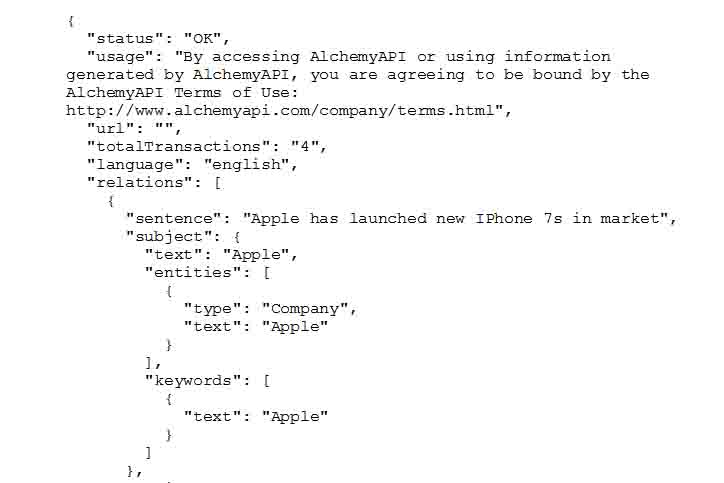
\includegraphics[width=13cm, height=9cm]{alchemy1}
	\centering
	\caption{An example of response format by Alchemy API Part1}
\end{figure}
\begin{figure}[h]
	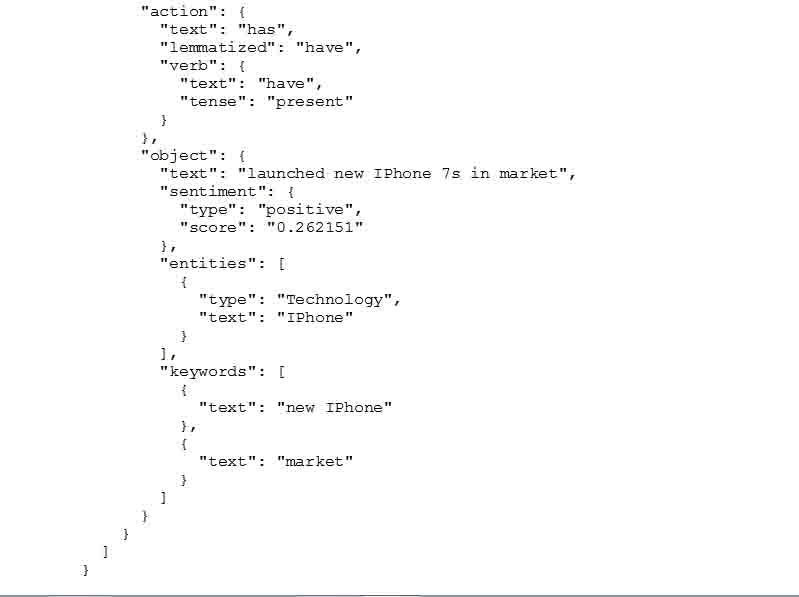
\includegraphics[width=13cm, height=9cm]{alchemy2}
	\centering
	\caption{An example of response format by Alchemy API Part2}
\end{figure}
\par 
The relations extracted from the article will be available in the form of triplets. It will be 	of the form \\(SUBJECT, OBJECT, VERB)
\begin{figure}[h]
	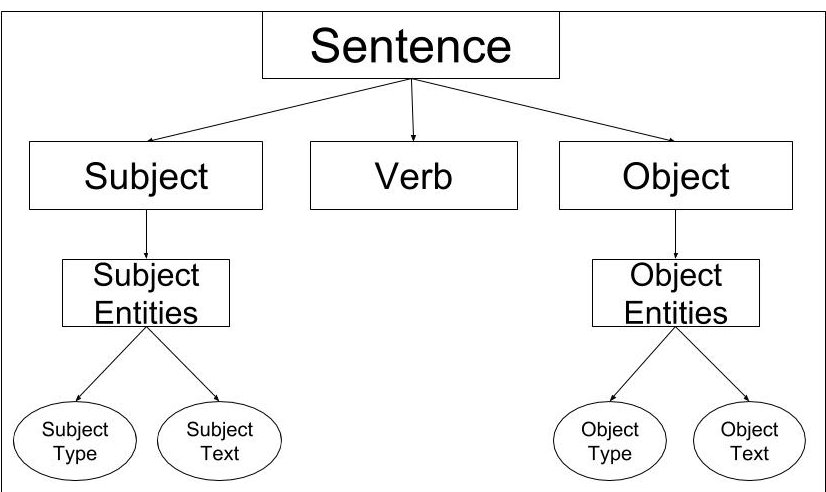
\includegraphics[width=13cm, height=7cm]{sentenceDiagram}
	\centering
	\caption{Extracted triplet relationship format}
\end{figure}
\par The subject field may consist of one on more entities depending upon the extracted relation. A subject entity will have a type (eg. Company) field and text (eg: Apple) field. Similar to the subject field, the object field too will have the type field and the text field. The third field, verb, is the entity that defines the relationship between the subject and the object. The verb term is also used to identify the context of the article.

\subsection{Validating the extracted relations}
\par Once a relation is extracted in the form of a triplet, it is needed to validate the relation before updating the relation to the data base. Two types of check are needed to be done 
. 
\begin{itemize}
\item Validation with grammar
\\ The relation triplet should be validated with the defined grammar syntaxes. If a matching syntax is encountered during the process, the relation will be validated.
\item Check for relation duplication
\\ There are chances that the currently extracted relation is already existing in the database. A search is done in the database for this purpose and if no matching relation is found existing already, the triplet will be validated for updation. 
\end{itemize}

\subsection{Tagging the articles}
\par Once a relationship triplet is extracted from the article and is checked for grammar validation, we need to properly tag the articles with related contexts and taxonomies to categorize the articles properly. Two methods of tagging is implemented in the system

\begin{itemize}
\item Context based tagging
\\ Context based tagging is done using the keywords extracted by the AlchemyAPI. For this purpose, each extracted keyword is searched for match in previously generated Context vocabulary. If a match is found, the article will be tagged with the concerned context.
\item Taxonomy based tagging
\\ Taxonomy based tagging is done using the verb terms identified by the API in the triplet extracted. A search is done in the Taxonomy vocabulary for match for each verb term. If found, the article will be tagged with the concerned taxonomy.
\end{itemize}

\section{Module 3 - Intermediate layer}
\par 
The intermediate layer used to pre-process the extracted relations, it removes the unwanted relations from getting added to the graph and the permanent relations table. This is done by presenting all the extracted relations for admin’s verification. Admin can select which one need to be added. After the admin approves the relation they are added to the graph database. Before adding to the graph it checked if the nodes involving the relation already exists if not they are created. Then the relation is added only if it doesn’t exist in the graph. Once the admin approves the relations are moved from temporary relations table

\section{Module 4 - Front end}
\par The three user interfaces as described in the web interface design is implemented using the following libraries.
\subsection{Bootstrap}
\par Bootstrap is a free and open-source front-end library for creating websites and web applications. It contains HTML- and CSS-based design templates for typography, forms, buttons, navigation and other interface components, as well as optional JavaScript extensions. It aims to ease the development of dynamic websites and web applications.\cite{bootstrap}
\begin{itemize}
\item Bootstrap is a front end web framework, that is, an interface for the user, unlike the server-side code which resides on the "back end" or server.
\item Bootstrap is the second most-starred project on GitHub, with over 95 thousand stars and more than 40 thousand forks.
\item Bootstrap is compatible with the latest versions of the Google Chrome, Firefox, Internet Explorer, Opera, and Safari browsers, although some of these browsers are not supported on all platforms.
\item Since version 2.0 it also supports responsive web design. This means the layout of web pages adjusts dynamically, taking into account the characteristics of the device used (desktop, tablet, mobile phone).
\item Starting with version 3.0, Bootstrap adopted a mobile-first design philosophy, emphasizing responsive design by default.
\item The version 4.0 alpha release added Sass and Flexbox support.
\item Bootstrap is open source and available on GitHub. Developers are encouraged to participate in the project and make their own contributions to the platform.
\end{itemize}

\subsection{D3.js}
\par D3.js is a JavaScript library for manipulating documents based on data. D3 helps you bring data to life using HTML, SVG, and CSS. D3’s emphasis on web standards gives you the full capabilities of modern browsers without tying yourself to a proprietary framework, combining powerful visualization components and a data-driven approach to DOM manipulation.
\par D3 allows you to bind arbitrary data to a Document Object Model (DOM), and then apply data-driven transformations to the document. For example, you can use D3 to generate an HTML table from an array of numbers. Or, use the same data to create an interactive SVG bar chart with smooth transitions and interaction.
\par D3 is not a monolithic framework that seeks to provide every conceivable feature. Instead, D3 solves the crux of the problem: efficient manipulation of documents based on data. This avoids proprietary representation and affords extraordinary flexibility, exposing the full capabilities of web standards such as HTML, SVG, and CSS. With minimal overhead, D3 is extremely fast, supporting large datasets and dynamic behaviours for interaction and animation. D3’s functional style allows code reuse through a diverse collection of components and plugins.
\subsection{Neod3}
Graph visualisation library for D3.js. This library a high-level abstraction of D3 graph rendering that let you produce beautiful, interactive graphs without having to know all the details.
\subsubsection{Usage}
\par The library primarily consists of two parts; graphModel, responsible for working with node and relationship data. And graphView, responsible for rendering and interacting with the graph.
\begin{lstlisting}
var graphModel = neo.graphModel()
  .nodes([
    {id: 0, labels: ['Person', 'Gamer'], properties: {name: "Johan"}},
    {id: 1, labels: ['Person'], properties: {name: "Sebastian"}}
  ])
  .relationships([
    {id: 0, source: 0, target: 1, type: 'KNOWS'}
  ])

var graphView = neo.graphView();

// Make sure you put an element with id=example in your DOM
d3.select("#example").datum(graphModel).call(graphView);
\end{lstlisting}
\par Let's add some interaction by adding a click handler to the graphView. The node argument is an instance of neo.model.Node. In this example, when a node is clicked, we create a new node, connect it with a relationship, and add it to the graph model. Either instantiate a new neo.model.Node, or use raw objects as we did in the initialization. The graphView listens to changes made to it's graphModel in the event handlers and automatically redraws the graph.
\begin{lstlisting}
var graphView = neo.graphView()
  .on('nodeClicked', function(node) {
    // Use objects as argument, e.g. neo.model.Node
    graphModel.nodes.add(new neo.model.Node(3, ['Person', 'Wannabe'], {name: 'Joel'}));

    // ...or use raw data
    graphModel.relationships.add({id: 2, source: node.id, target: 3, type: 'KNOWS'});
  })
;
\end{lstlisting}
\par 
Note that all calls are chainable so you can just keep adding handlers. Let's add one that removes a relationship when clicked, and removes a node when double-clicked. Note that remove accepts both identifiers and objects.
\begin{lstlisting}
  .on('onRelationshipClicked', function(relationship) {
    graphModel.relationships.remove(relationship);
  })
  .on('onNodeDblClicked', function(node) {
    graphModel.nodes.remove(node.id);
  })
;
\end{lstlisting}
\par So far we've rendered the graph with the build-in default styling. Let's add some custom styling by loading a GraSS stylesheet. First create the stylesheet:
\begin{lstlisting}
/* style.grass */
node {
  diameter: 40px;
  color: #DFE1E3;
  border-color: #D4D6D7;
  border-width: 2px;
  text-color-internal: #000000;
  caption: '{name}';
  font-size: 10px;
}

relationship {
  color: #D4D6D7;
  shaft-width: 1px;
  font-size: 8px;
  padding: 3px;
  text-color-external: #000000;
  text-color-internal: #FFFFFF;
}
\end{lstlisting}
\par In this example we load the stylesheet from your server. Since loading of files is performed asynchronously, we'll need to do the initialization in the XHR response callback.

\begin{lstlisting}
d3.xhr("style.grass", "application/grass", function(request) {
  var graphView = neo.graphView()
    // .on( ...
    .style(request.responseText)
  ;

  d3.select("#example").datum(graphModel).call(graphView);
});
\end{lstlisting}
\subsection{For the naive user}
\par 
The list of all articles that has been fetched by Dynamic data collector is listed here for the naïve user’s reference this is categorized according to their tags.  A synopsis of the article is provided in here itself, the interested user can follow the link to the original article. This feature is provided as an add-on, since all the data about the fetched articles has been saved in the postgres database, it will only cause minimal overhead and provide utility service for the naïve user. Bootstrap has been used to implemented this web user interface.
\subsection{For the business user}
\par The business user can query the graph database to get a variety of predefined relations. The results may be shown either as the graph visualization or as a tabular representation according to the type of query. The graph visualization is implemented using neod3 graph visualization library. 
\subsection{For the administrator}
\par The administrator interface lists the relations that are extracted by the Dynamic data extractor. Each relations will have subject, subject type, object, object type predicate, and predicate type. The sentence from which these relations are extracted are shown for verification. This will allow the filtering of duplicate as well as junk data.

\chapter{Testing and Results}
\section{Unit testing}
Unit test procedures were conducted after the development of each module, reviewed and verified for correspondence to component level design. The data extraction module was tested to ensure that only the required data is collected. We also made sure that the data we collected are in our expected format. . All of the unit test cases covered the interface to the module to ensure proper flow of data, the local data structures used to ensure integrity of data during execution and boundary conditions. Input combinations were chosen to exercise all independent paths and error handling paths. The following were the unit test cases designed and implemented:
\subsection{Web Interfaces}
\subsubsection{Search Module}
Test cases were designed to ensure that all relationships are displayed. Tests made sure that when the fields are empty and when no relationship exists for a node appropriate “search unsuccessful” messages are shown. Tests were conducted to ensure that failure messages are display upon any failures due to error in connection to databases.
\subsubsection{Process Node module}
Test cases were designed to ensure that nodes are properly added and deleted from the database It was ensured that the Node Table and graph database was updated whenever a node was added or deleted .Tests were also conducted to ensure that unsuccessful and failure messages are shown accordingly.
\subsubsection{Process Relationship module}
Test cases were designed to ensure that relationships were inserted deleted and updated correctly. It was also ensured that empty fields displayed error messages. Failure and unsuccessful message paths were also exercised.

\section{Integration Testing}
Integration testing is a systematic technique for constructing the program structure while conducting tests to uncover errors associated with interfacing. The objective is to take the unit tested modules and build a program structure that has been dictated by design.
Incremental integration testing was followed. The strategy used was bottom up integration. It was implemented in the following way:
\begin{itemize}
\item The data extraction module and the NLP module were integrated to form a cluster. The data correctly extracted was stored in the PostgreSQL database.
\item Output from the cluster was fed into the middleware module, in which the taxonomy classification was performed.
\item Next part of testing was integrating the output of the middleware module with the Graph database. The graph was displayed in the web interface.
\end{itemize}
Each time a new module was added, regression testing was performed. This involved re-testing the previously tested modules by re-execution of some of the subsets of tests that had already been performed to ensure that the addition of new modules has not led to unintended side effects. 

\section{Validation testing}
\par
A series of black box tests were conducted to ensure that all functional requirements were satisfied, all behavioral characteristics were achieved and all performance requirements were attained. Conformity to reasonable expectations outlined in the Software Requirements Specifications under validation criteria was checked with.It was ensured that all the web pages were directed correctly from one page to another in case of the web interface provided. 
\paragraph*{Alpha and beta testing}The alpha version of the application was tested by the teachers and the other students who were not part of this team. The beta version of the application has not yet been launched.

\section{System Testing}
System testing is actually a series of different tests whose primary purpose is to fully exercise the computer based system. The following types of systems tests were performed.
\section{Recovery Testing}
Recovery testing is a system test that forces the system to fail in a variety of ways and verifies that recovery is properly performed. In this case the system was forced to fail in variety of ways for example by disconnecting PostgreSQL while still retaining connections to graph database. It was ensured that in all such situations the system is consistent.
\section{Performance Testing}
For real time systems, software that provides the required functions but does not conform to performance requirements is unacceptable. Thus run-time performance test of software within the context of an integrated system is very important. Performance testing was done at all stages of the development of this project. Performance of each individual module was tested individually and it was verified that each module conforms to the requirements. After this all the modules were integrated and tested. The database was expanded sufficiently to verify that the performance does not degrade with increase in data.
\section{Results}
\subsection{Final Application}
\subsubsection{Web Interface}
\begin{figure}[h]
	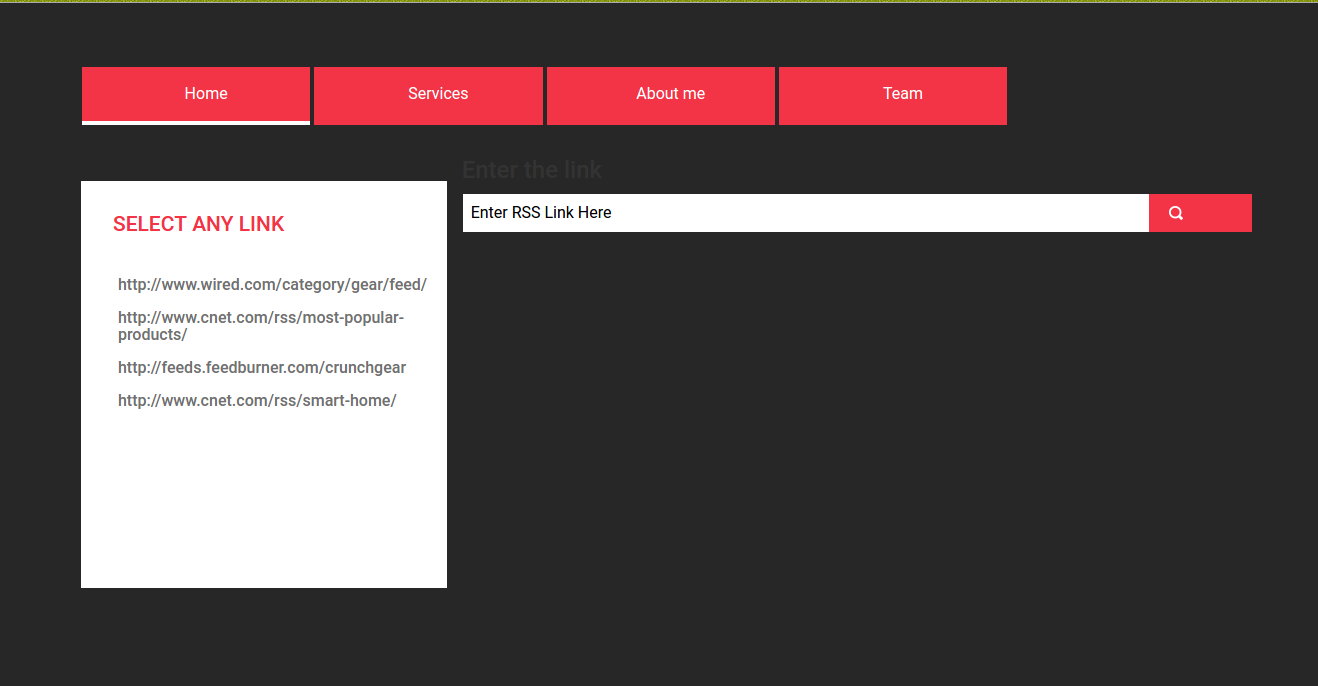
\includegraphics[width=13cm, height=8cm]{naiveUser}
	\centering
	\caption{Interface provided for the naïve user}
	\label{fig:naiveUser}
\end{figure}
Interface provided for the naïve user is shown in figure \ref{fig:naiveUser}. User can enter the link of the RSS feed he need to inspect, or he can select any of the links we have provided.

\begin{figure}[h]
	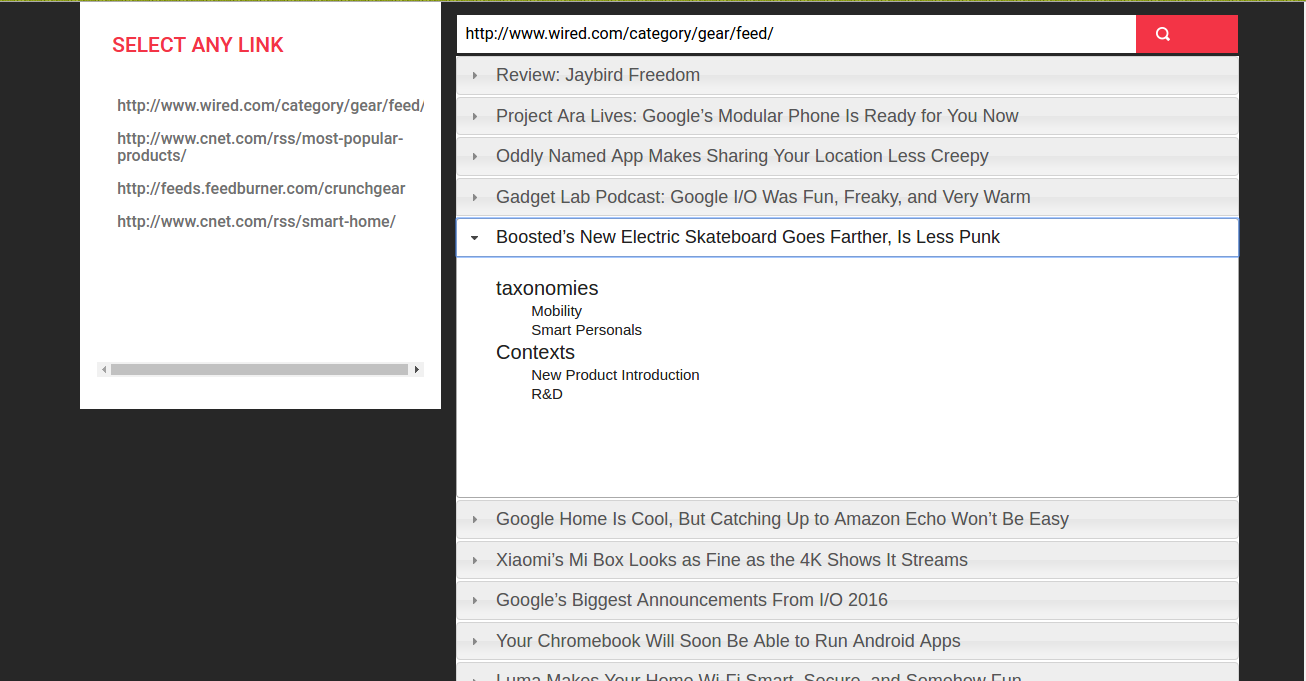
\includegraphics[width=13cm, height=8cm]{naiveUserContent}
	\centering
	\caption{Screenshot of the page when content of a link is extracted}
	\label{fig:naiveUserContent}
\end{figure}
The figure \ref{fig:naiveUserContent} shows the screenshot when the content of a link is extracted.

\begin{figure}[h]
	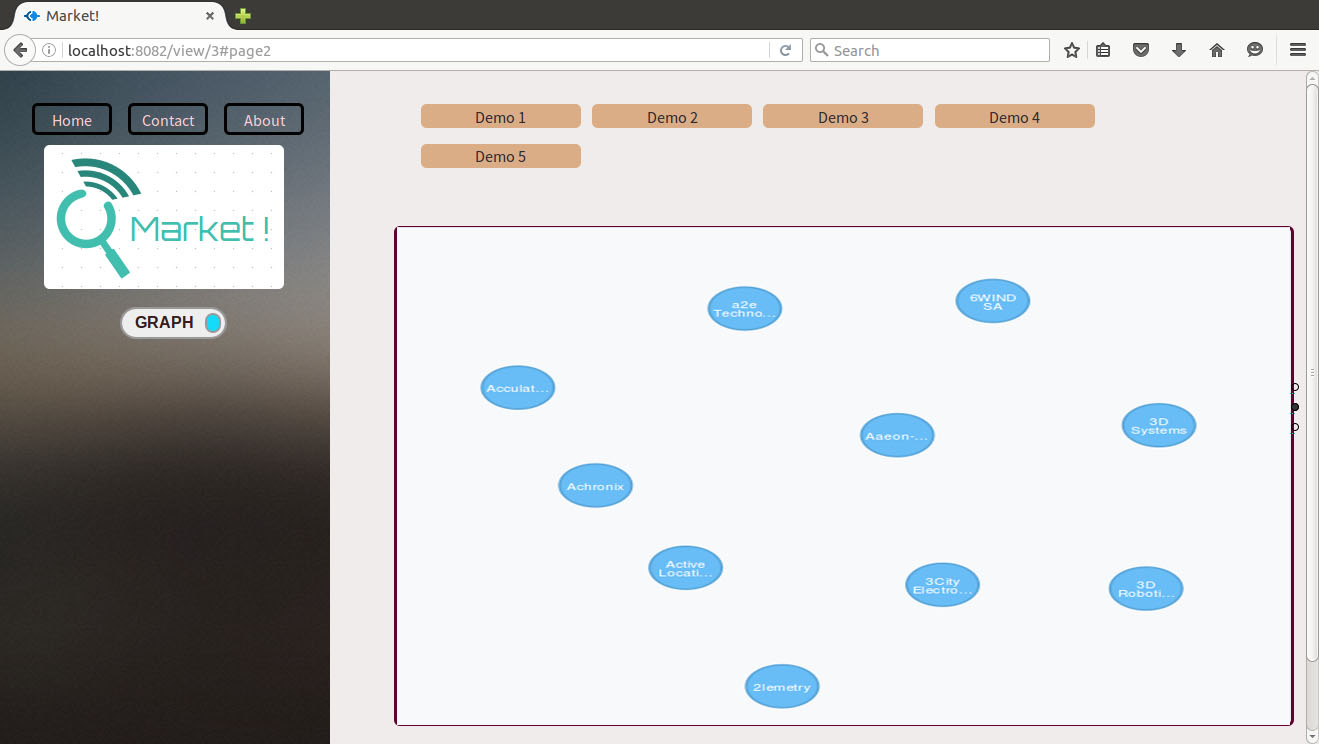
\includegraphics[width=13cm, height=8cm]{queryDatabase}
	\centering
	\caption{Screenshot of the page when user to query the graph database}
	\label{fig:queryDatabase}
\end{figure}
The figure \ref{fig:queryDatabase} shows screenshot of the interface used by the user to query the graph database and see the results.
\paragraph*{D3 Visualizations}
\begin{figure}[h]
	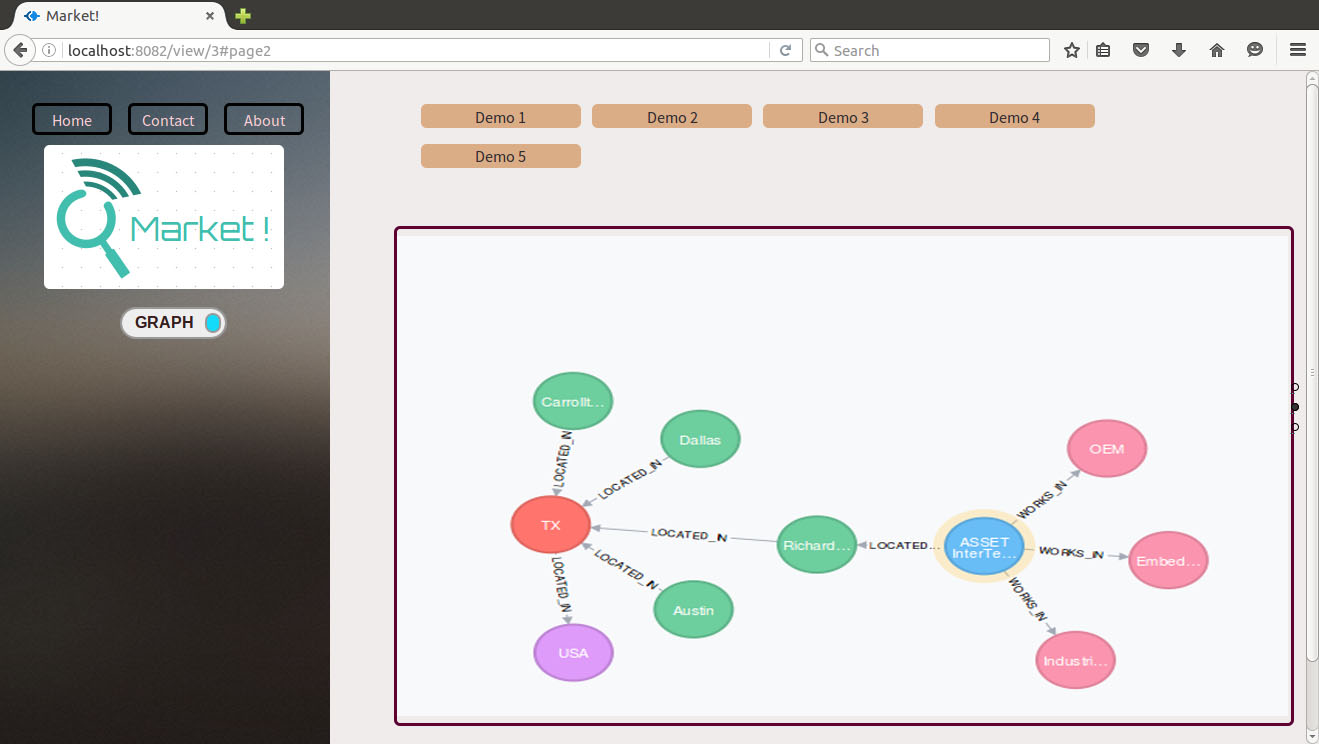
\includegraphics[width=13cm, height=8cm]{d3visual1}
	\centering
	\caption{Example Query: Querying of Asset Technologies}
	\label{fig:d3visual1}
\end{figure}
Figure \ref{fig:d3visual1} shows the screenshot which displays the query of Asset Technologies. It locations, area of expertise are displayed as nodes.
\begin{figure}[h]
	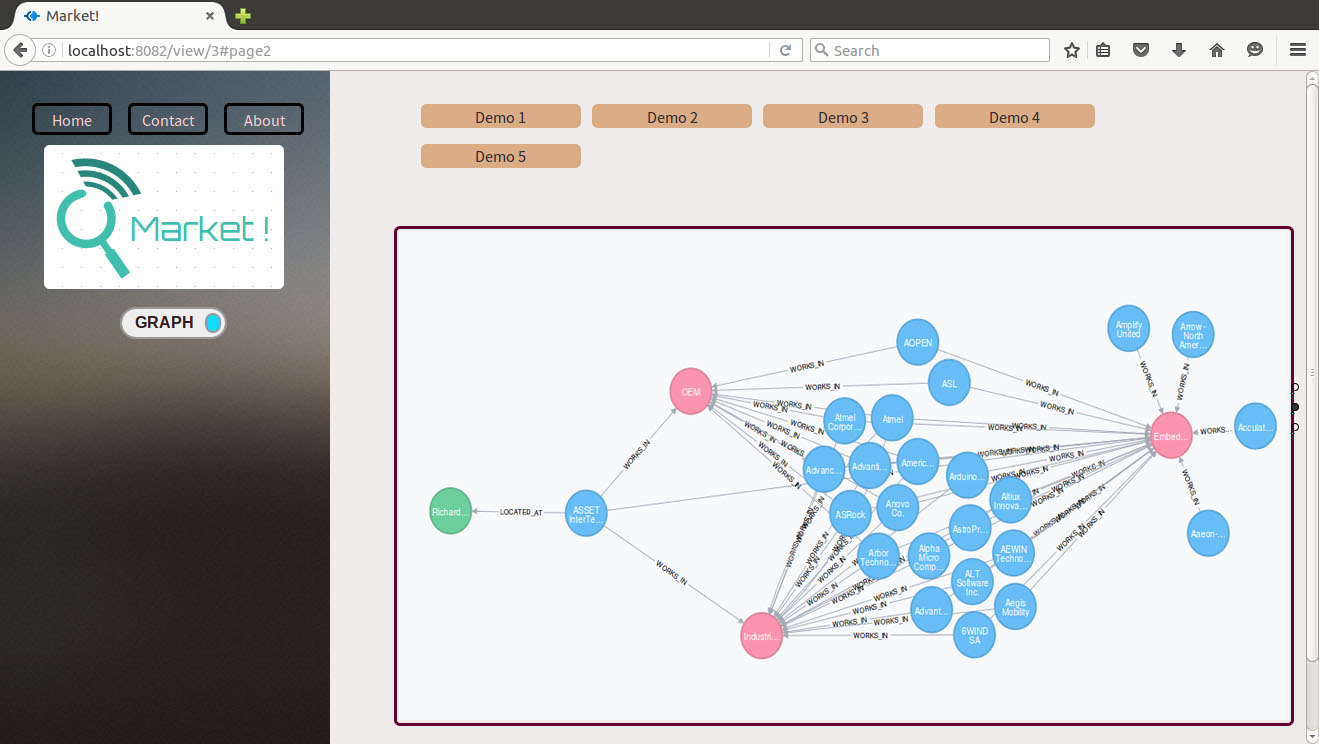
\includegraphics[width=13cm, height=8cm]{d3visual2}
	\centering
	\caption{Example Query: Expanding Nodes}
	\label{fig:d3visual2}
\end{figure}
Figure \ref{fig:d3visual2} shows the screenshot which displays the nodes of OEM, Industrial technology and Embedded technology when expanded.

\begin{figure}[h]
	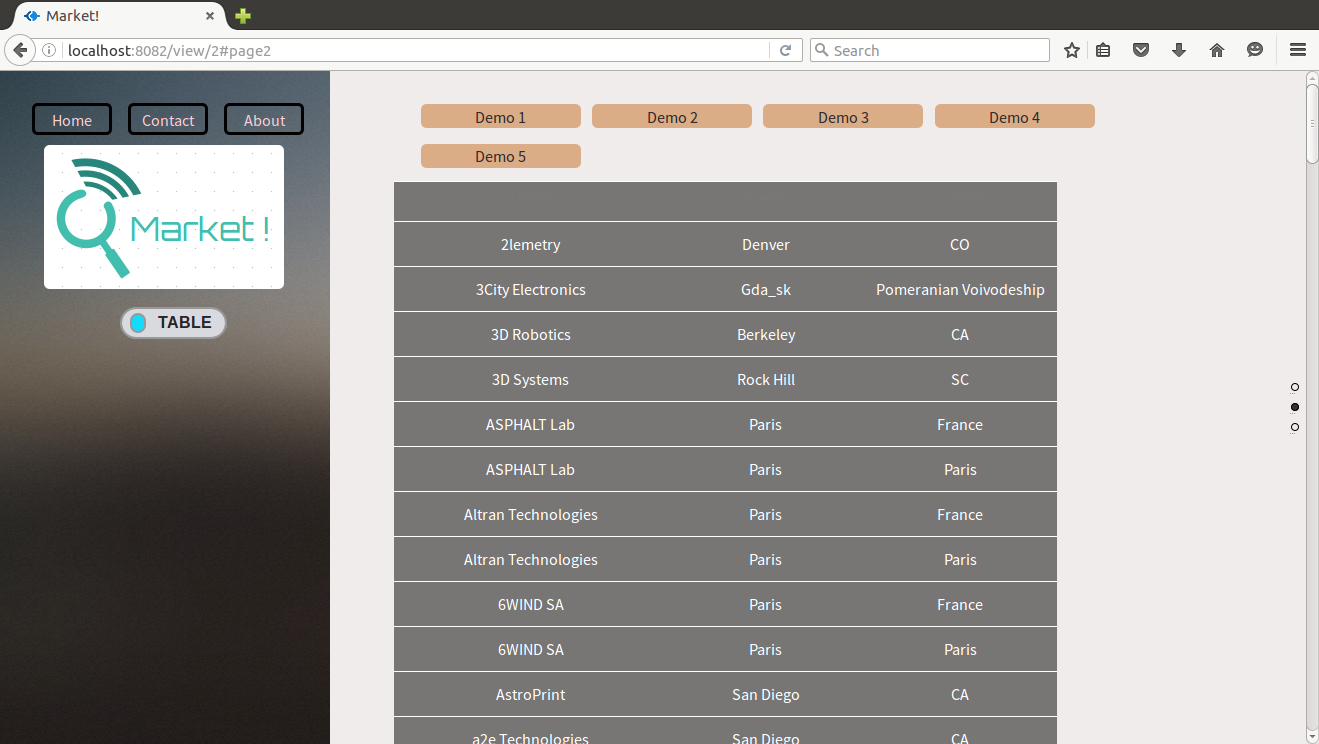
\includegraphics[width=13cm, height=8cm]{tableview}
	\centering
	\caption{Example Query: Companies Locations}
	\label{fig:tableview}
\end{figure}
Figure \ref{fig:tableview} shows the screenshot which displays table visualization of a query.


\begin{figure}[h]
	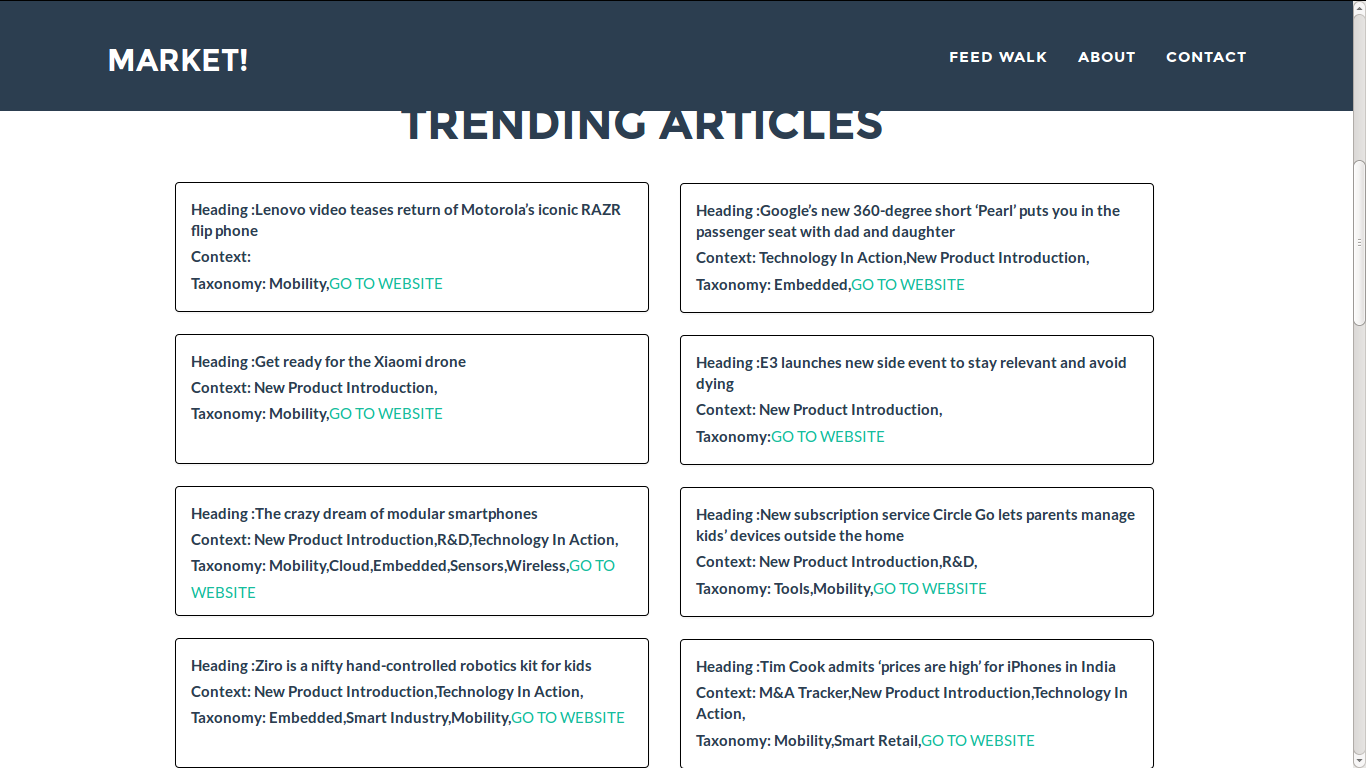
\includegraphics[width=13cm, height=8cm]{newsarticles}
	\centering
	\caption{website diplays latest query information}
	\label{fig:newsarticles}
\end{figure}
Figure \ref{fig:newsarticles} shows the screenshot of the website which provide the latest technology related information.

\end{document}	

